\newpage
\section*{Esempi}
\subsection*{Immagini}

\begin{figure}[h]
    \centering
    \begin{subfigure}[]{0.5\linewidth}
    \centering
    
\includegraphics[scale=0.2]{img/pittogrammi/Acute toxicity.png}
    \caption{Acute toxicity}
    \end{subfigure}
    \begin{subfigure}[]{0.5\linewidth}
    \centering
    
\includegraphics[scale=0.2]{img/pittogrammi/Explosive.png}
    \caption{Explosive}
    \end{subfigure}
    \caption{Due immagini incolonnate al centro della pagina con posizione h definita da te.}
    \label{fig:1}
\end{figure}

\textit{Lorem ipsum dolor sit amet, consectetur adipiscing elit. Maecenas eget nisl elementum, pretium libero suscipit, interdum tellus. Praesent luctus commodo massa, vel molestie augue laoreet ac. Phasellus sodales auctor erat eu porta. Donec at volutpat nunc. Phasellus pretium, eros vitae cursus ornare, turpis massa egestas sem, ut varius ipsum metus nec mi. Integer ut odio erat. Interdum et malesuada fames ac ante ipsum primis in faucibus. Sed finibus, tortor in tristique iaculis, odio tortor finibus nisi, nec varius felis justo eu tortor. Interdum et malesuada fames ac ante ipsum primis in faucibus. Donec ultrices in ante vel imperdiet. Ut porttitor consectetur sodales. Vestibulum ante ipsum primis in faucibus orci luctus et ultrices posuere cubilia curae; Nullam non neque quis tortor convallis pulvinar id vel libero.}

\begin{figure}[!h]
\floatbox[{\capbeside\thisfloatsetup{capbesideposition={right,top},capbesidewidth=0.45\textwidth}}]{figure}[\FBwidth]
{\caption{didascalia dell'immagine centrale con didascalia a fianco.}}
{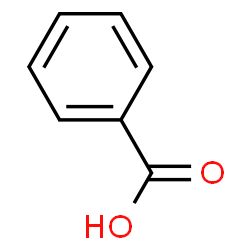
\includegraphics[width=0.1\textwidth]{img/acbenz.png}}
{\label{fig:2}}
\end{figure}

\textit{Aliquam erat nulla, suscipit id dignissim molestie, eleifend quis tortor. Pellentesque tempus egestas orci, sit amet eleifend elit condimentum id. Etiam id nisi velit. Etiam mauris nisl, facilisis sed egestas nec, tempor a est. In eget lacus vitae velit volutpat maximus. Vestibulum maximus arcu sit amet lacus maximus consequat. Duis sodales libero non metus finibus, eget ornare sem consequat.}

\begin{wrapfigure}{r}{0.3\textwidth} %this figure will be at the right
    \centering
    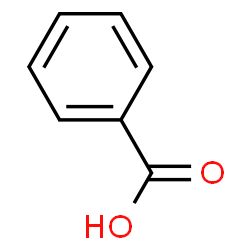
\includegraphics[scale=0.5]{img/acbenz.png}
    \caption{Didascalia dell'immagine sulla destra circondata da testo.} 
    \label{fig:3}
\end{wrapfigure}

\textit{Nullam vel lorem porttitor, convallis ex eget, condimentum velit. Integer sed sem aliquet, elementum ipsum in, rutrum elit. Vestibulum in arcu eget odio egestas varius. Vivamus lacus augue, dignissim at arcu a, consequat iaculis leo. Nam sit amet varius tellus. Nulla tempor velit nibh, et tincidunt diam porta vel. Mauris sit amet erat ut neque vehicula ultrices et eu sem. Phasellus pellentesque ultricies sapien. Curabitur at sodales mauris, maximus auctor mi. Vestibulum semper mauris in euismod rutrum. Fusce pellentesque in mi ac euismod.}

\textit{Nam gravida magna ut volutpat placerat. Pellentesque habitant morbi tristique senectus et netus et malesuada fames ac turpis egestas. Sed consequat justo condimentum metus bibendum mattis. Etiam id euismod ante. Nam sit amet ex libero. Proin id mauris at neque pellentesque accumsan eu ut ligula. Vivamus sodales magna sed risus faucibus tincidunt in eu felis.}

\begin{figure}
    \centering
    
\includegraphics[scale=0.2]{img/pittogrammi/Acute toxicity.png}
    
\includegraphics[scale=0.2]{img/pittogrammi/Explosive.png}
    \caption{Figure affiancate al centro della pagina nella posizione decisa da LaTex}
    \label{fig:4}
\end{figure}

\textit{Vivamus sit amet suscipit turpis, at eleifend risus. Vestibulum ante ipsum primis in faucibus orci luctus et ultrices posuere cubilia curae; Curabitur eget pharetra est, in mattis erat. Aenean pharetra finibus posuere. Nullam ipsum lacus, molestie nec eros eu, lacinia facilisis augue. Aenean dapibus rhoncus mi ut vulputate. Mauris commodo ultricies nulla egestas porttitor.}

\begin{figure}[h]
    \centering
    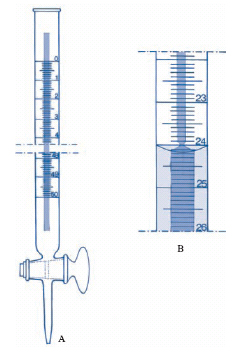
\includegraphics{img/buretta.jpg}
    \caption{Buretta}
    \label{fig:5}
\end{figure}

\newpage
\subsection*{Formule chimiche}
\begin{figure}[!ht]
    \chemfig{O=H}
\end{figure}

\begin{figure}[!ht]
    \chemfig{A-[1]B-[7]C}
    \caption{To define chemical formulae you can use units that define the angles}
\end{figure}

\begin{figure}[!ht]
    \chemfig{A-[:50]B-[:-25]C}
    \caption{Absolute angles}
\end{figure}


\begin{figure}[!ht]
    \chemfig{A-[::50]B-[::-25]C}
    \caption{Relative angles}
\end{figure}


\begin{figure}[!ht]
    \chemfig{A*5(-B=C-D-E=)}
    \caption{Regular polygons}
\end{figure}

\begin{figure}[!ht]
    \chemfig{A*5(-B=C-D)}
    \caption{Incomplete rings are also possible}
\end{figure}

\begin{figure}[!ht]
    \chemfig{H-C(-[2]H)(-[6]H)-C(=[1]O)-[7]H}
    \caption{Branched molecule}
\end{figure}

\begin{figure}
    \chemfig{A*6(-B=C(-CH_3)-D-E-F(=G)=)}
    \caption{Branched ring}
\end{figure}

\begin{figure}[!ht]
{\huge 
    \setchemfig{atom sep=2em,bond style={line width=1pt,red,dash pattern=on 2pt off 2pt}}  
    \chemname
    {\chemfig{H-C(-[2]H)(-[6]H)-C(=[1]O)-[7]H}}    
    {Ethanal}
}
\end{figure}

\newpage
\subsection*{Molecular orbital diagrams}
\begin{figure}[!ht]
        \begin{modiagram}
        \atom{left}{1s, 2s, 2p}
        \end{modiagram}
    \caption{First molecular orbital diagrams}
\end{figure}

\begin{figure}[!ht]
\begin{modiagram}
 \atom{right}{
    1s = { 0; pair} ,
    2s = { 1; pair} ,
    2p = {1.5; up, down }
 }


 \atom{left}{
    1s = { 0; pair} ,
    2s = { 1; pair} ,
    2p = {1.5; up, down }
 }
 \end{modiagram}
 \end{figure}

\begin{figure}[!ht]
 \begin{modiagram}
 \atom{left}{1s}
 \atom{right}{1s={;up}}
 \molecule{
    1sMO={0.75;pair,up}
  }
\end{modiagram}
\end{figure}

\begin{figure}[!ht]
\begin{modiagram}
 \atom{left}{
      1s, 2s, 2p = {;pair,up,up}
  }
  \atom{right}{
      1s, 2s, 2p = {;pair,up,up}
  }
  \molecule{
      1sMO, 2sMO, 2pMO = {;pair,pair,pair,up,up}
  }
\end{modiagram}
\end{figure}

\begin{figure}[!ht]
\begin{modiagram}
 \atom{left}{1s}
 \atom{right}{1s={;up}}
 \molecule{
    1sMO={;pair,up}
 }
 \draw[<-,shorten <=8pt,shorten >=15pt,blue]
 (1sigma*) --++(2,1) node {anti-bonding MO};
\end{modiagram}
\end{figure}

\newpage
\subsection*{Flowchart}
Ecco invece un esempio di flowchart che potrebbe essere utile in certi procedimenti particolarmente articolati.
\begin{figure}[!ht]
    \begin{center}
        \begin{tikzpicture}[node distance=2cm] % per guida -> https://it.overleaf.com/learn/latex/LaTeX_Graphics_using_TikZ%3A_A_Tutorial_for_Beginners_(Part_3)%E2%80%94Creating_Flowcharts
            \node (start) [startstop] {Inizio};
            \node (in1) [io, below of=start] {Ingresso};
            \node (pro1) [process, below of=in1] {Processo 1};
            \node (dec1) [decision, below of=pro1,  yshift=-0.5cm] {Decsione 1};
            \node (pro2a) [process, below of=dec1, yshift=-0.5cm] {Process 2a};
            \node (pro2b) [process, right of=dec1, xshift=2cm] {Process 2b};
            \node (out1) [io, below of=pro2a] {Output};
            \node (stop) [startstop, below of=out1] {Stop};
            
            \draw [arrow] (start) -- (in1);
            \draw [arrow] (in1) -- (pro1);
            \draw [arrow] (pro1) -- (dec1);
            \draw [arrow] (dec1) -- node[anchor=east] {yes} (pro2a);
            \draw [arrow] (dec1) -- node[anchor=south] {no} (pro2b);
            \draw [arrow] (pro2b) |- (pro1); %per fare linea segmentata
            \draw [arrow] (pro2a) -- (out1);
            \draw [arrow] (out1) -- (stop);
        \end{tikzpicture}
    \end{center}
\end{figure}

\newpage
\subsection*{Note e appunti vari}
Lorem ipsum dolor sit amet, consectetur adipiscing elit. Sed eget velit ullamcorper, convallis neque eget, tempus leo. Aenean eget est ornare, mattis turpis sit amet, vestibulum ante.\unsure{Change this!} Integer quis molestie arcu. Duis sem felis, posuere ut ante vitae, lobortis tincidunt dolor. Ut aliquet nunc sed lorem vehicula, ac tristique velit venenatis. Aliquam feugiat interdum magna, luctus sodales velit porta et. Nunc varius lorem nec varius malesuada. Praesent ante nisi, ultrices et venenatis sed, commodo vitae eros.\change{Change this!}

Pellentesque consectetur malesuada lectus, ut faucibus diam egestas ac. Aenean porttitor at libero a venenatis. Morbi sollicitudin, leo sed pellentesque facilisis, lacus diam lobortis tellus, sit \info{This can help me in chapter seven!}amet vulputate turpis sem id ipsum. Nunc ac aliquet mi, non porta quam. Maecenas auctor pulvinar sodales. Suspendisse eget mi arcu. Mauris quis nulla sit amet risus dapibus eleifend sed eget purus. Pellentesque libero nunc, \improvement{This really needs to be improved!\newline\newline What was I thinking?!}congue vitae mi sit amet, lobortis faucibus ante. Vestibulum cursus, neque quis auctor laoreet, sapien risus vestibulum orci, a rutrum tellus nisl quis ligula.

Sed non erat metus. Donec aliquet ex non neque sodales pretium. Aliquam eu sapien elit. Aliquam finibus felis et neque elementum, laoreet tempus urna auctor. Vivamus ac congue elit, vitae volutpat nulla. Sed pretium in lorem eget porttitor. Etiam interdum euismod odio, quis sollicitudin tellus rutrum et. Proin consequat, risus at consequat elementum, turpis elit tincidunt tellus, eu finibus dui mi vel eros. Donec in nulla tortor. Maecenas mollis consectetur erat sed elementum. Pellentesque habitant morbi tristique senectus et netus et malesuada fames ac turpis egestas. Nunc ultrices enim ut risus scelerisque, sed ultrices nibh congue. Mauris volutpat, elit vel sagittis consequat, lorem sapien iaculis sapien, id faucibus purus eros ut mauris. Vestibulum ornare elementum pretium.

Nunc non ante suscipit, dictum justo nec, dapibus elit. Proin lacinia leo fermentum dui bibendum, ac pellentesque felis malesuada. Integer sollicitudin tempor varius. Quisque sed magna rhoncus, ultricies nisi a, sollicitudin quam. Curabitur ut tempor lectus. Donec iaculis condimentum vehicula. In convallis ac sapien vel aliquam. Orci varius natoque penatibus et magnis dis parturient montes, nascetur ridiculus mus. Suspendisse ac eleifend dolor, at scelerisque urna. Quisque ac facilisis erat. Etiam accumsan risus sed molestie pulvinar. Orci varius natoque penatibus et magnis dis parturient montes, nascetur ridiculus mus. Proin non turpis non felis pretium convallis.
\improvement[inline]{The following section needs to be rewritten!}

Sed finibus pellentesque diam, et sagittis tortor ultrices ut. Orci varius natoque penatibus et magnis dis parturient montes, nascetur ridiculus mus. Suspendisse volutpat ullamcorper dui in cursus. Proin ullamcorper neque posuere porttitor rutrum. Suspendisse ac tortor justo. Vivamus convallis ligula at lacus commodo, eu mattis nulla vehicula. Vestibulum interdum leo et volutpat rhoncus.
\thiswillnotshow{This is hidden since option `disable' is chosen!}

E ora aggiungo una lista delle note.
\listoftodos[Notes to address]